\documentclass[10pt, aspectratio=169]{beamer}

% --- Packages ---
\usepackage{booktabs}
\usepackage{amsmath}
\usepackage{amsfonts}
\usepackage{amssymb}
\usepackage{enumitem}
\usepackage{tikz}
\usepackage{pgfplots}
\usepackage{listings}
\usepackage{xcolor}
\usepackage[most]{tcolorbox}

% Defining the greenbox environment
\newtcolorbox{greenbox}{
    colback=green!5!white, 
    colframe=green!40!black, 
    sharp corners=southwest, 
    boxrule=0.5pt,
    left=2pt, right=2pt, top=2pt, bottom=2pt
}

% Let Overleaf automatically figure out the highest pgfplots version it can support
\pgfplotsset{compat=newest} 
\usetikzlibrary{shapes.geometric, arrows.meta, positioning, calc, fit, backgrounds, shapes.misc}

% --- Universal Internal Theme Switch ---
\usetheme{metropolis} 

% --- Safe Custom Color Definitions ---
% We define them cleanly using xcolor so Beamer doesn't trip over the '#' character
\definecolor{CodeBg}{HTML}{EDF2F7}
\definecolor{CodeText}{HTML}{2C3E50}
\definecolor{CodeKeyword}{HTML}{2B6CB0}
\definecolor{CodeString}{HTML}{16A085}
\definecolor{CodeComment}{HTML}{718096}

% --- Code Styling ---
\lstset{
    basicstyle=\ttfamily\scriptsize\color{CodeText},
    backgroundcolor=\color{CodeBg},
    frame=single,
    rulecolor=\color{CodeBg},
    breaklines=true,
    keywordstyle=\color{CodeKeyword},
    stringstyle=\color{CodeString},
    commentstyle=\color{CodeComment}
}

% --- Title Info ---
\title{Supervised Fine-Tuning (SFT)}
\subtitle{Teaching LLMs to Formulate Text \& Follow Instructions}
\author{SFT from A to Z}
\date{\the\year}

\begin{document}

% --- Slide 1: Title ---
\begin{frame}[plain]
	\maketitle
\end{frame}

% --- Slide 2: Pre-training vs SFT ---
\begin{frame}{Pre-training vs. SFT (The Mindset Shift)}
	\begin{columns}[T]
		\begin{column}{0.48\textwidth}
			\centering
			\textbf{Base LLM (Text Completer)}
			\vskip 0.5em
			\begin{minipage}{\textwidth}
				\scriptsize
				\textbf{Prompt:} Write a python function for quicksort.\\
				\textbf{Completion:} Quicksort was invented by Tony Hoare in 1959. It is a divide-and-conquer algorithm. The complexity is $O(n \log n)$...
			\end{minipage}
			\vskip 1em
			
\begin{tikzpicture}
				\node[draw=red!60, fill=red!5, rounded corners, inner sep=6pt, text width=0.9\textwidth, align=center] {
					\scriptsize \textbf{Chaos Pattern}: Fails to answer the intent; naively predicts the next statistically likely web tokens.
				};
			\end{tikzpicture}
		\end{column}

		\begin{column}{0.04\textwidth}
			\centering
			\vline width 0.5pt height 4cm
		\end{column}

		\begin{column}{0.48\textwidth}
			\centering
			\textbf{SFT LLM (Helpful Assistant)}
			\vskip 0.5em
			\begin{minipage}{\textwidth}
				\scriptsize
				\textbf{Prompt:} Write a python function for quicksort.\\
				\textbf{Completion:} Here is the quicksort implementation:\\
				\texttt{def quicksort(arr):... return arr}
			\end{minipage}
			\vskip 2em
			
\begin{tikzpicture}
				\node[draw=green!60, fill=green!5, rounded corners, inner sep=6pt, text width=0.9\textwidth, align=center] {
					\scriptsize \textbf{Alignment Pattern}: Transitions from pure raw completion to playing the persona of an assistant.
				};
			\end{tikzpicture}
		\end{column}
	\end{columns}
\end{frame}

% --- Slide 3: Pipeline ---
\begin{frame}{The LLM Alignment Pipeline}
	\centering
	\vskip 0.5cm
	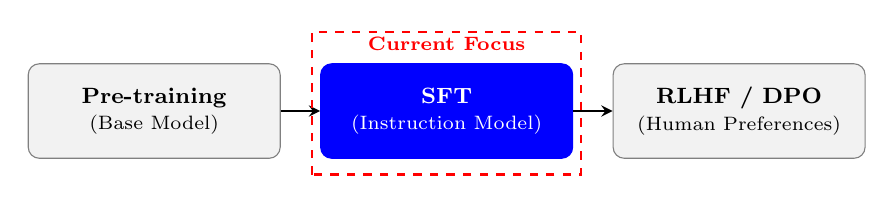
\begin{tikzpicture}[node distance=0.5cm, every node/.style={font=\footnotesize}]
		\node (pt) [draw=gray, fill=gray!10, minimum width=3.2cm, minimum height=1.2cm, align=center, rounded corners]
		{\textbf{Pre-training}\\ \scriptsize (Base Model)};

		\node (sft) [draw=blue, fill=blue, text=white, minimum width=3.2cm, minimum height=1.2cm, align=center, rounded corners, right=of pt]
		{\textbf{SFT}\\ \scriptsize (Instruction Model)};

		\node (rlhf) [draw=gray, fill=gray!10, minimum width=3.2cm, minimum height=1.2cm, align=center, rounded corners, right=of sft]
		{\textbf{RLHF / DPO}\\ \scriptsize (Human Preferences)};

		\draw[thick, ->, >=stealth] (pt) -- (sft);
		\draw[thick, ->, >=stealth] (sft) -- (rlhf);

		\draw[thick, dashed, color=red] ($(sft.south west)+(-0.1,-0.2)$) rectangle ($(sft.north east)+(0.1,0.4)$);
		\node[color=red, font=\scriptsize\bfseries] at ($(sft.north)+(0,0.25)$) {Current Focus};
	\end{tikzpicture}
	\vfill
	\begin{itemize}
		\item \textbf{Pre-training:} Web-scale raw knowledge and language structure acquisition ($10^{12}+$ tokens)
		\item \textbf{SFT:} Teaching interaction formats, tasks, and system behaviors ($10^4 - 10^5$ examples)
		\item \textbf{RLHF/DPO:} Micro-tuning behavior to meet safety standards and human feedback
	\end{itemize}
\end{frame}

% --- Slide 4: Tradeoff ---
\begin{frame}{Prompt Engineering vs. SFT: The Core Tradeoff}
	\centering
	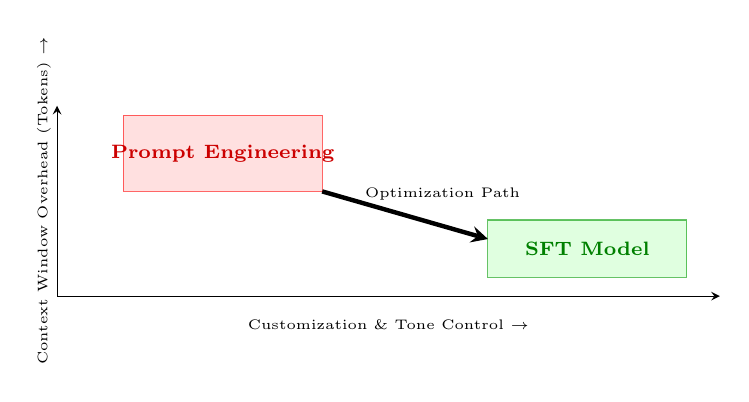
\begin{tikzpicture}
		\begin{axis}[
				width=10cm, height=4.0cm,
				xlabel={Customization \& Tone Control $\rightarrow$},
				ylabel={Context Window Overhead (Tokens) $\rightarrow$},
				xmin=0, xmax=10,
				ymin=0, ymax=10,
				ticks=none,
				axis lines=left,
				every axis y label/.style={at={(axis description cs:-0.02,0.5)},rotate=90,anchor=center, font=\tiny},
				every axis x label/.style={at={(axis description cs:0.5,-0.15)},anchor=center, font=\tiny},
			]
			% Prompting Zone
			\draw[fill=red!20, draw=red, opacity=0.6] (axis cs:1,5.5) rectangle (axis cs:4,9.5);
			\node[color=red!80!black, font=\scriptsize\bfseries] at (axis cs:2.5,7.5) {Prompt Engineering};

			% SFT Zone
			\draw[fill=green!20, draw=green!60!black, opacity=0.6] (axis cs:6.5,1) rectangle (axis cs:9.5,4);
			\node[color=green!50!black, font=\scriptsize\bfseries] at (axis cs:8,2.5) {SFT Model};

			% Optimization Vector Arrow
			\draw[ultra thick, ->, >=stealth, color=black] (axis cs:4,5.5) -- (axis cs:6.5,3);
			\node[font=\tiny, anchor=south west] at (axis cs:4.5,4.5) {Optimization Path};
		\end{axis}
	\end{tikzpicture}

	\vskip 0.5em

	% Direct Head-to-Head Comparison Table
	\scriptsize
	\begin{table}
		\centering
		\begin{tabular}{lll}
			\toprule
			\textbf{Metric}             & \textbf{\color{red!80!black}Prompt Engineering (Few-Shot)} & \textbf{\color{green!50!black}Supervised Fine-Tuning (SFT)} \\
			\midrule
			\textbf{Upfront Cost}       & \textbf{\$0} (Immediate setup via API)                     & \textbf{High} (Data collection + GPU rent)                  \\
			\textbf{Cost Per Request}   & \textbf{High} (Paying for examples every time)             & \textbf{Minimal} (Short, clean prompts)                     \\
			\textbf{Format Reliability} & Weak (Model can drift or forget rules)                     & Hardcoded (Baked into model weights)                        \\
			\bottomrule
		\end{tabular}
	\end{table}
\end{frame}

% --- Slide 5: Anatomy ---
\begin{frame}[fragile]{The Anatomy of an Instruction Dataset}

	\begin{block}{ChatML / OpenAI JSON Template Structure}
		% Part 1: System and User lines (Transparent background)
		\begin{lstlisting}[belowskip=-0.8em]
[
  {"role": "system", "content": "You are a helpful coding assistant."},
  {"role": "user", "content": "How do I reverse a list in Python?"},
        \end{lstlisting}

		% Part 2: Assistant line (Wrapped in a custom multi-line tcolorbox container)
		\vskip -0.2cm
		\begin{tcolorbox}[
				colback=orange!15,
				colframe=orange!15,
				arc=0mm,
				boxrule=0pt,
				left=0mm, right=5mm, top=0mm, bottom=1mm,
				grow to left by=0.1cm, grow to right by=0.1cm
			]
			\begin{lstlisting}[
                backgroundcolor=\color{orange!15}, 
                frame=none, 
                aboveskip=0em, 
                belowskip=0em, 
                breaklines=true, 
                breakatwhitespace=true
            ]
  {"role": "assistant", "content": "You can reverse a list using `list.reverse()` or slicing `[::-1]`."}
            \end{lstlisting}
		\end{tcolorbox}

		% Part 3: Closing bracket (Transparent background)
		\vskip -0.2cm
		\begin{lstlisting}
]
        \end{lstlisting}
	\end{block}

	% Clear text note placed safely below the code block
	\vskip 0.1cm
	\begin{center}
		\color{orange!90!black}\footnotesize\bfseries
		$\uparrow$ The Gold Target (Loss is calculated ONLY on the highlighted Assistant response)
	\end{center}
	\vskip 0.1cm

	% Bottom part: Detailed structural roles documentation
	\begin{columns}[T]
		\begin{column}{0.4\textwidth}
			\centering
			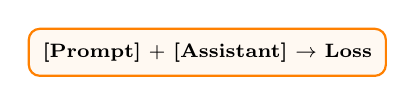
\begin{tikzpicture}
				\node[draw=orange, thick, rounded corners, inner sep=5pt, fill=orange!5] {
					\scriptsize \textbf{[Prompt]} + \textbf{[Assistant]} $\rightarrow$ \textbf{Loss}
				};
			\end{tikzpicture}
		\end{column}
		\begin{column}{0.6\textwidth}
			\small
			\textbf{System:} Defines boundaries/tone. \\
			\textbf{User:} Input instructions. \\
			\textbf{Assistant:} The training target.
		\end{column}
	\end{columns}
\end{frame}

% --- Slide 6: Quality Over Quantity ---
\begin{frame}{Quality Over Quantity: The LIMA Effect}
	\begin{columns}[c]

		% Left Column: The TikZ Data Scaling Graph
		\begin{column}{0.58\textwidth}
			\centering
			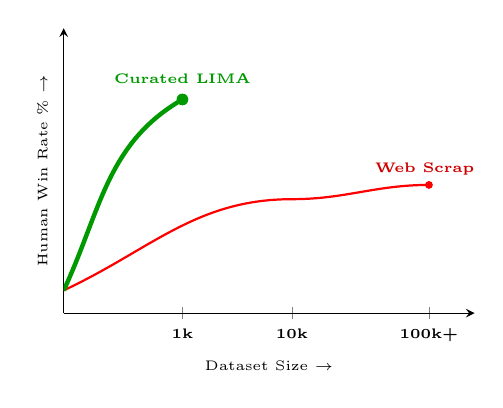
\begin{tikzpicture}
				\begin{axis} [
						width=6.8cm, height=5.2cm,
						xlabel={Dataset Size $\rightarrow$},
						ylabel={Human Win Rate \% $\rightarrow$},
						ylabel style={font=\tiny},
						xlabel style={font=\tiny},
						xmin=0.5, xmax=5.0,
						ymin=0, ymax=10,
						axis lines=left,
						xtick={1.8, 3.0, 4.5},
						xticklabels={1k, 10k, 100k+},
						xticklabel style={font=\tiny\bfseries},
						ytick=\empty
					]
					% Curve 1: Low-quality uncurated Web Scraped Data
					\draw[thick, red] (axis cs:0.5,0.8) to[out=25,in=180] (axis cs:3.0,4) to[out=0,in=180] (axis cs:4.5,4.5);
					\node[color=red!80!black, font=\tiny\bfseries, anchor=south] at (axis cs:4.5,4.5) {Web Scraps};
					\node[circle, fill=red, inner sep=1pt] at (axis cs:4.5,4.5) {};

					% Curve 2: High-quality Curated Data (LIMA approach)
					\draw[ultra thick, green!60!black] (axis cs:0.5,0.8) to[out=65,in=210] (axis cs:1.8,7.5);
					\node[color=green!60!black, font=\tiny\bfseries, anchor=south] at (axis cs:1.8,7.7) {Curated LIMA};
					\node[circle, fill=green!60!black, inner sep=1.5pt] at (axis cs:1.8,7.5) {};
				\end{axis}
			\end{tikzpicture}
		\end{column}

		% --- Right Column: Manually formatted definition block ---
		\begin{column}{0.40\textwidth}
			\begin{greenbox}
				% Manually styling the title to ensure it displays correctly
				\textcolor{green!40!black}{\textbf{Definition: Human Win Rate}}
				\vskip 0.1cm
				\scriptsize
				An evaluation metric where human experts run blind A/B tests to compare two anonymous model outputs for the exact same prompt.
				\vskip 0.15cm
				\textbf{How it works:}
				\begin{itemize}
					\item \textbf{Input:} Same prompt given to Model A and Model B.
					\item \textbf{Evaluation:} Human judges pick the superior answer.
					\item \textbf{Metric:} If Model A wins 75 out of 100 matchups, its Win Rate is \textbf{75\%}.
				\end{itemize}
			\end{greenbox}
		\end{column}
	\end{columns}

	\vskip 0.2cm

	% Bottom block remains full width to summarize the paradigm
	\begin{block}{The Core SFT Dataset Paradigm}
		\vspace{0.15cm}
		\scriptsize
		The famous \textbf{LIMA (Less Is More for Alignment)} study demonstrated that a tiny set of 1,000 meticulously filtered, high-quality instruction responses consistently outperforms massive, multi-thousand sample datasets full of token noise, structural typos, and repetitive language model patterns.
	\end{block}
\end{frame}

% --- Slide 7: Synthetic ---
\begin{frame}{Data Synthetic Generation (Self-Instruct)}
	\centering
	\vskip 0.5cm
	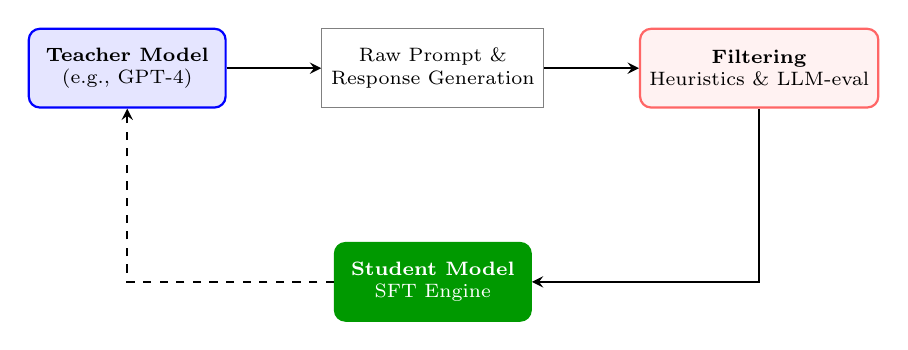
\begin{tikzpicture}[node distance=1.2cm, every node/.style={font=\scriptsize}]
		\node (teacher) [draw=blue, fill=blue!10, thick, minimum width=2.5cm, minimum height=1cm, align=center, rounded corners]
		{\textbf{Teacher Model}\\(e.g., GPT-4)};

		\node (gen) [draw=gray, fill=white, right=of teacher, minimum width=2.5cm, minimum height=1cm, align=center]
		{Raw Prompt \&\\Response Generation};

		\node (filter) [draw=red!60, fill=red!5, thick, right=of gen, minimum width=2.5cm, minimum height=1cm, align=center, rounded corners]
		{\textbf{Filtering}\\Heuristics \& LLM-eval};

		\node (student) [draw=green!60!black, fill=green!60!black, text=white, below=of gen, yshift=-0.5cm, minimum width=2.5cm, minimum height=1cm, align=center, rounded corners]
		{\textbf{Student Model}\\SFT Engine};

		\draw[thick, ->, >=stealth] (teacher) -- (gen);
		\draw[thick, ->, >=stealth] (gen) -- (filter);
		\draw[thick, ->, >=stealth] (filter) |- (student);
		\draw[thick, ->, >=stealth, dashed] (student) -| (teacher);
	\end{tikzpicture}
	\vfill
	\begin{itemize}
		\item \textbf{Pipeline:} Seed tasks $\rightarrow$ Generation loops $\rightarrow$ Deduplication checks $\rightarrow$ Target training.
		\item \textbf{Pitfall:} Risk of data echo chambers; repeating systemic hallucination footprints of the teacher.
	\end{itemize}
\end{frame}

\begin{frame}{The Necessity of Chat Templates}
	\textbf{The Challenge: Text Completion vs. Interaction}
	\begin{itemize}
		\item \textbf{Base Model Behavior:} Predicts the next word in a sequence. Without structure, it treats a prompt as a \textit{continuation} of a text (e.g., finishing your question).
		\item \textbf{The Goal:} Turn an open-ended generator into a controlled \textit{dialogue agent}.
	\end{itemize}

	\vskip 0.8em
	\begin{columns}[T]
		% Слева: Ожидание (Структура)
		\begin{column}{0.48\textwidth}
			\textbf{Expectation (Controlled)}
			\begin{tcolorbox}[colback=green!5, colframe=green!20, boxrule=0.5pt]
				\ttfamily\scriptsize
				\textcolor{blue!70!black}{User:} 4+4?\\
				\textcolor{blue!70!black}{Assistant:} \textcolor{green!20!black}{8}\\
				\textcolor{gray}{[STOP TOKEN]}
			\end{tcolorbox}
		\end{column}

		% Справа: Реальность (Role Bleeding)
		\begin{column}{0.48\textwidth}
			\textbf{Reality (Uncontrolled)}
			\begin{tcolorbox}[colback=red!5, colframe=red!20, boxrule=0.5pt]
				\ttfamily\scriptsize
				\textcolor{blue!70!black}{User:} 4+4?\\
				\textcolor{blue!70!black}{Assistant:} \textcolor{green!20!black}{8\\
					\textbf{User: And what is 5+5?}\\
					\textbf{Assistant: 10}} \\
				\textcolor{gray}{[STOP TOKEN]}
			\end{tcolorbox}
		\end{column}
	\end{columns}
\end{frame}

% --- Slide 8: Pitfalls ---
\begin{frame}{The Solution: Chat Templates}
	\textbf{Enforcing boundaries with Special Tokens}

	\vskip 1em
	\begin{tcolorbox}[colback=green!5, colframe=green!20, coltitle=black, title=Model respects the structure]
		\ttfamily\scriptsize
		<|im\_start|>User: What is 4+4?<|im\_end|> \\
		\textcolor{green!60!black}{<|im\_start|>Assistant: 8<|im\_end|>}
	\end{tcolorbox}

	\vskip 1em
	\begin{itemize}
		\item \textbf{Containment:} The model is confined to the green scope.
		\item \textbf{Control:} The \colorbox{gray!15}{\texttt{<|im\_end|>}} tag serves as an explicit "Stop" signal for the tokenizer.
	\end{itemize}

	\vskip 0.5em
	\begin{block}{\textbf{Crucial Technical Step:}}
		Tags must be registered as \textbf{Special Tokens} to prevent fragmentation. \\
		\textit{Fix:} \colorbox{gray!15}{\texttt{tokenizer.add\_special\_tokens()}} $\rightarrow$ \colorbox{gray!15}{\texttt{model.resize\_token\_embeddings()}}.
	\end{block}
\end{frame}

% --- Slide 9: Loss ---
\begin{frame}{Standard SFT Loss Function}
	\centering
	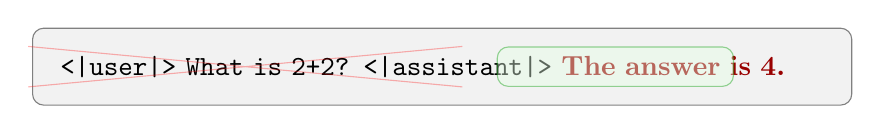
\begin{tikzpicture}
		\node[draw=gray, fill=gray!10, rounded corners, inner sep=10pt, text width=0.8\textwidth, align=left] {
			\texttt{<|user|> What is 2+2? <|assistant|>} \color{red!60!black}\textbf{The answer is 4.}
		};
		\node[draw=red, fill=red!10, cross out, minimum width=5.5cm, minimum height=0.5cm, opacity=0.3] at (-2.5,0) {};
		\node[draw=green!60!black, fill=green!10, rounded corners, minimum width=3cm, minimum height=0.5cm, opacity=0.4] at (2.2,0) {};
	\end{tikzpicture}
	\vskip 1em
	\begin{equation*}
		\mathcal{L} = -\sum_{t=i}^{N} \log P(x_t \mid x_{<t}) \quad \text{where } i \text{ is the first token of the assistant's answer}
	\end{equation*}
	\vskip 0.5em
	\begin{itemize}
		\item \textbf{Masked Multi-turn Loss:} Only the assistant's response contributes to the loss.
		\item \textbf{Gradient Flow:} Backpropagation is constrained to target tokens, forcing the model to learn answer generation, not prompt replication.
	\end{itemize}
\end{frame}

% --- Slide 10: Full vs PEFT ---
\begin{frame}{Full Fine-Tuning vs. PEFT}
	\begin{columns}[T]
		\begin{column}{0.48\textwidth}
			\centering
			\textbf{Full Fine-Tuning (FT)}
			\vskip 1em
			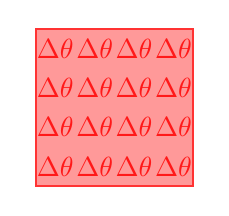
\begin{tikzpicture}[scale=0.5]
				\draw[fill=red!40, draw=red!80, thick] (0,0) rectangle (4,4);
				\foreach \x in {0.5,1.5,2.5,3.5}
				\foreach \y in {0.5,1.5,2.5,3.5}
				\node[color=red!90] at (\x,\y) {$\Delta\theta$};
			\end{tikzpicture}
			\vskip 1em
			\scriptsize Modifies \textbf{every single parameter}. High risk of catastrophic forgetting. Massive VRAM requirements to maintain gradients and optimizer states.
		\end{column}

		\begin{column}{0.04\textwidth}
			\centering
			\vline width 0.5pt height 4cm
		\end{column}

		\begin{column}{0.48\textwidth}
			\centering
			\textbf{PEFT (LoRA)}
			\vskip 1em
			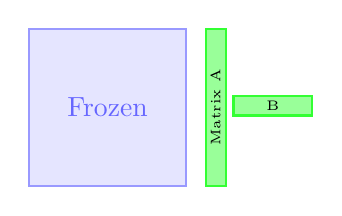
\begin{tikzpicture}[scale=0.5]
				\draw[fill=blue!10, draw=blue!40, thick] (0,0) rectangle (4,4);
				\node at (2,2) {\color{blue!60}Frozen};

				\draw[fill=green!40, draw=green!80, thick] (4.5,0) rectangle (5,4);
				\node[rotate=90, font=\tiny] at (4.75,2) {Matrix A};

				\draw[fill=green!40, draw=green!80, thick] (5.2,1.8) rectangle (7.2,2.3);
				\node[font=\tiny] at (6.2,2.05) {B};
			\end{tikzpicture}
			\vskip 1.5em
			\scriptsize \textbf{PEFT (Parameter-Efficient Fine-Tuning)}
			\vskip 0.5em
			\scriptsize \textbf{Strategy:} Train only a tiny fraction of parameters. Base model remains locked ($99\%+$ frozen).
			\vskip 0.5em
			\scriptsize \textbf{LoRA (Low-Rank Adaptation):}
			\scriptsize Injects trainable matrices $A, B$ into layers. Represents updates as low-rank decomposition: $\Delta W = AB$.
		\end{column}
	\end{columns}
\end{frame}

% --- Slide 11: LoRA Math ---
\begin{frame}{Inside LoRA (Low-Rank Adaptation)}
	\begin{columns}[T]
		% Left Column: Parameters and Comparison Table
		\begin{column}{0.275\textwidth}
			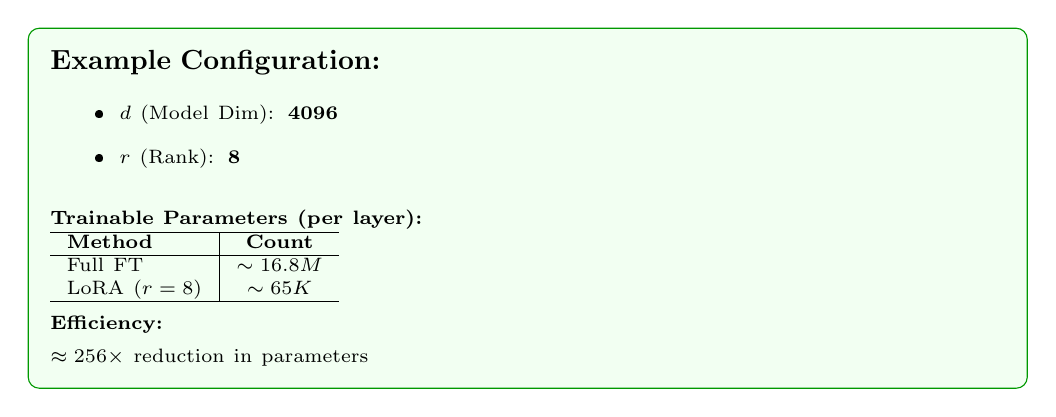
\begin{tikzpicture}
				\node[draw=green!60!black, fill=green!5, rounded corners, inner sep=8pt, text width=\textwidth] {
					\textbf{Example Configuration:} \\
					\scriptsize
					\begin{itemize}
						\item $d$ (Model Dim): \textbf{4096}
						\item $r$ (Rank): \textbf{8}
					\end{itemize}
					\vskip 0.5em
					\textbf{Trainable Parameters (per layer):} \\
					\scriptsize
					\begin{tabular}{l|c}
						\hline
						\textbf{Method} & \textbf{Count} \\ \hline
						Full FT         & $\sim 16.8M$   \\
						LoRA ($r=8$)    & $\sim 65K$     \\ \hline
					\end{tabular}
					\vskip 0.5em
					\textbf{Efficiency:} \\
					\scriptsize $\approx 256\times$ reduction in parameters
				};
			\end{tikzpicture}
		\end{column}
		\begin{column}{0.725\textwidth}
			\centering
			\Large
			\begin{equation*}
				W_{\text{updated}} = W_0 + \Delta W = W_0 + \frac{\alpha}{r} (B \times A)
			\end{equation*}
			\vskip 0.8cm
			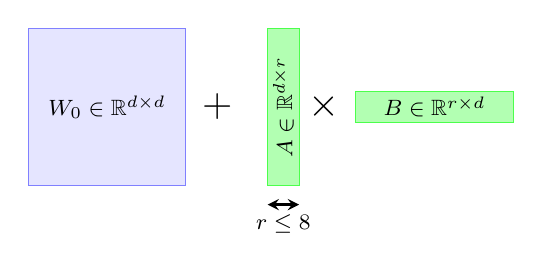
\begin{tikzpicture}[scale=0.8, every node/.style={font=\footnotesize}]
				\draw[fill=blue!10, draw=blue!50] (0,0) rectangle (2.5,2.5);
				\node at (1.25,1.25) {$W_0 \in \mathbb{R}^{d \times d}$};

				\node at (3,1.25) {\Large $+$};

				\draw[fill=green!30, draw=green!70] (3.8,0) rectangle (4.3,2.5);
				\node[rotate=90] at (4.05,1.25) {$A \in \mathbb{R}^{d \times r}$};

				\node at (4.7,1.25) {\Large $\times$};

				\draw[fill=green!30, draw=green!70] (5.2,1.0) rectangle (7.7,1.5);
				\node at (6.45,1.25) {$B \in \mathbb{R}^{r \times d}$};

				\draw[thick, <->, >=stealth] (3.8, -0.3) -- (4.3, -0.3);
				\node at (4.05, -0.6) {$r \le 8$};
			\end{tikzpicture}
		\end{column}
	\end{columns}
	\vfill
	\begin{itemize}
		\scriptsize
		\item \textbf{Assumption:} Target adjustments $\Delta W$ feature highly reduced intrinsic rank dimensional limits during training.
		\item \textbf{Setup:} Matrix A defaults to standard Gaussian distributions; Matrix B initializes at zero. This guarantees $\Delta W = 0$ at step zero.
	\end{itemize}
\end{frame}

% --- Slide 12: Quantization ---
\begin{frame}{Memory Layout: Quantization \& QLoRA}
	\centering
	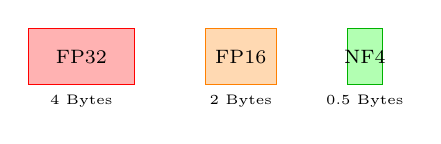
\begin{tikzpicture}[scale=0.9]
		\draw[fill=red!30, draw=red] (0,1.8) rectangle (1.5,2.6);
		\node at (0.75,2.2) {\scriptsize FP32};
		\node[below] at (0.75,1.8) {\tiny 4 Bytes};

		\draw[fill=orange!30, draw=orange] (2.5,1.8) rectangle (3.5,2.6);
		\node at (3,2.2) {\scriptsize FP16};
		\node[below] at (3,1.8) {\tiny 2 Bytes};

		\draw[fill=green!30, draw=green!70!black] (4.5,1.8) rectangle (5,2.6);
		\node at (4.75,2.2) {\scriptsize NF4};
		\node[below] at (4.75,1.8) {\tiny 0.5 Bytes};
	\end{tikzpicture}
	\vskip 0.5cm
	\textbf{VRAM Footprint Matrix for a Standard 7B Parameter Model:}
	\vskip 0.5em
	\begin{table}
		\scriptsize
		\centering
		\begin{tabular}{llll}
			\toprule
			\textbf{Precision Mode} & \textbf{Data Format}        & \textbf{Model Weights Footprint} & \textbf{Total VRAM Needed for SFT}     \\
			\midrule
			Full Precision          & FP32                        & $\sim$ 28 GB                     & $\sim$ 112 GB (including states)       \\
			Half Precision          & FP16 / BF16                 & $\sim$ 14 GB                     & $\sim$ 40-50 GB                        \\
			\textbf{QLoRA}          & \textbf{NF4 (NormalFloat4)} & \textbf{$\sim$ 4.5 GB}           & \textbf{$<$ 8 GB (Consumer-grade GPU)} \\
			\bottomrule
		\end{tabular}
	\end{table}
\end{frame}

% --- Slide 13: Hyperparameters ---
\begin{frame}{Hyperparameters That Actually Matter}
	\begin{columns}[T]
		\begin{column}{0.31\textwidth}
			\centering
			\textbf{Learning Rate}
			\vskip 0.5em
			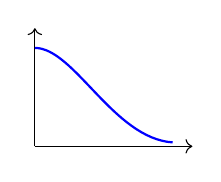
\begin{tikzpicture}[scale=0.5]
				\draw[->] (0,0) -- (4,0);
				\draw[->] (0,0) -- (0,3);
				\draw[thick, color=blue] (0,2.5) .. controls (1,2.5) and (2,0.2) .. (3.5,0.1);
			\end{tikzpicture}
			\vskip 0.5em
			\tiny
			\textbf{Cosine Decay Schedule}\\
			\vskip 0.5em
			$\sim 1e-4$ for LoRA runs.\\
			$\sim 2e-5$ for Full FT runs.\\
			Magnitudes lower than foundational pre-training rates.
		\end{column}

		\begin{column}{0.02\textwidth}
			\vline width 0.2pt height 4cm
		\end{column}

		\begin{column}{0.31\textwidth}
			\centering
			\textbf{Batch Size}
			\vskip 1em
			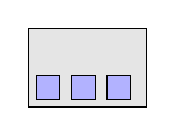
\begin{tikzpicture}[scale=0.5]
				\draw[draw=black, fill=gray!20] (0,0) rectangle (3,2);
				\draw[fill=blue!30] (0.2,0.2) rectangle (0.8,0.8);
				\draw[fill=blue!30] (1.1,0.2) rectangle (1.7,0.8);
				\draw[fill=blue!30] (2.0,0.2) rectangle (2.6,0.8);
			\end{tikzpicture}
			\vskip 1em
			\tiny
			\textbf{Global vs. Per-device}\\
			\vskip 0.5em
			\textbf{Effective Batch Size:} The number of samples processed before updating weights (Target: 32--128).\\
			\vskip 0.5em
			\textbf{Gradient Accumulation:} If your GPU is too small for the target batch, process data in mini-batches and sum the gradients. Only update weights after the "effective" batch size is reached.
		\end{column}

		\begin{column}{0.02\textwidth}
			\vline width 0.2pt height 4cm
		\end{column}

		\begin{column}{0.31\textwidth}
			\centering
			\textbf{Context Strategy}
			\vskip 1.5em
			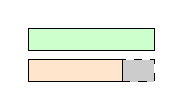
\begin{tikzpicture}[scale=0.4]
				\draw[fill=green!20] (0,1.5) rectangle (4,2.2);
				\draw[fill=orange!20] (0,0.5) rectangle (3,1.2);
				\draw[fill=gray!40, dashed] (3,0.5) rectangle (4,1.2);
			\end{tikzpicture}
			\vskip 1.5em
			\tiny
			\textbf{Packing vs. Padding}\\
			\vskip 0.5em
			\textbf{Padding}: Wastes tensor space via zero allocation.\\
			\vskip 0.5em
			\textbf{Packing}: Chains short strings sequentially separated by EOS tokens to maximize sequence efficiency.
		\end{column}
	\end{columns}
\end{frame}

% --- Slide 14: Overfitting ---
\begin{frame}{Fine-tuning Challenges: Overfitting \& Forgetting}
	\begin{columns}[T]
		% --- Column 1: Overfitting ---
		\begin{column}{0.48\textwidth}
			\begin{block}{1. Overfitting}
				Model memorizes noise instead of patterns.
			\end{block}
			\centering
			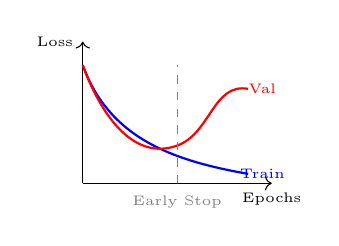
\begin{tikzpicture}[scale=0.6]
				\draw[->] (0,0) -- (4,0) node[below] {\tiny Epochs};
				\draw[->] (0,0) -- (0,3) node[left] {\tiny Loss};
				\draw[blue, thick] (0,2.5) to[out=-70, in=170] (3.5,0.2);
				\node[blue, font=\tiny] at (3.8,0.2) {Train};
				\draw[red, thick] (0,2.5) to[out=-70, in=200] (2,0.8) to[out=20, in=170] (3.5,2.0);
				\node[red, font=\tiny] at (3.8,2.0) {Val};
				\draw[dashed, gray] (2,0) -- (2,2.5);
				\node[font=\tiny, gray] at (2,-0.4) {Early Stop};
			\end{tikzpicture}

			\vspace{0.2cm}
			\alert{Solution: Early Stopping}
		\end{column}

		% --- Column 2: Forgetting ---
		\begin{column}{0.48\textwidth}
			\begin{block}{2. Catastrophic Forgetting}
				New skills override base general intelligence.
			\end{block}

			\vspace{0.3cm}
			\centering
			% Visual for Rehearsal (5-10% Anchor)
			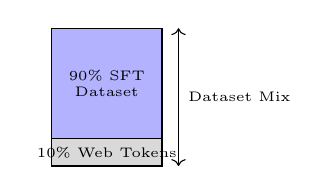
\begin{tikzpicture}[scale=0.7]
				% Stacked bar representation
				\draw[fill=gray!30] (0,0) rectangle (2,0.5) node[midway, font=\tiny] {10\% Web Tokens};
				\draw[fill=blue!30] (0,0.5) rectangle (2,2.5) node[midway, font=\tiny, align=center] {90\% SFT\\Dataset};
				\draw[<->] (2.3,0) -- (2.3,2.5) node[midway, right, font=\tiny] {Dataset Mix};
			\end{tikzpicture}

			\vspace{0.6cm}
			\alert{Mitigation: Data Rehearsal}
		\end{column}
	\end{columns}
\end{frame}

% --- Slide 15: Evaluation ---
\begin{frame}{How to Evaluate an SFT Model?}
	\centering
	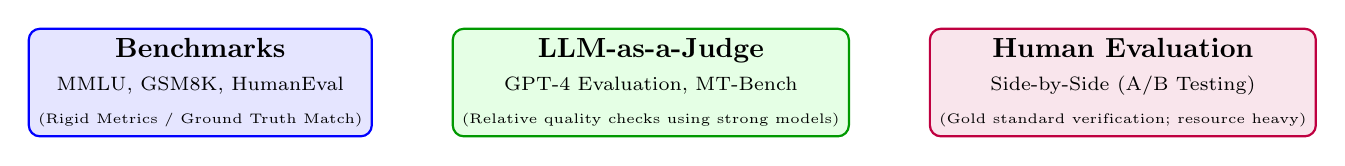
\begin{tikzpicture}[node distance=1cm]
		\node (bench) [draw=blue, fill=blue!10, thick, rounded corners, minimum width=3.5cm, minimum height=1.2cm, align=center] {
			\textbf{Benchmarks}\\
			\scriptsize MMLU, GSM8K, HumanEval\\
			\tiny (Rigid Metrics / Ground Truth Match)
		};

		\node (judge) [draw=green!60!black, fill=green!10, thick, rounded corners, minimum width=3.5cm, minimum height=1.2cm, align=center, right=of bench] {
			\textbf{LLM-as-a-Judge}\\
			\scriptsize GPT-4 Evaluation, MT-Bench\\
			\tiny (Relative quality checks using strong models)
		};

		\node (human) [draw=purple, fill=purple!10, thick, rounded corners, minimum width=3.5cm, minimum height=1.2cm, align=center, right=of judge] {
			\textbf{Human Evaluation}\\
			\scriptsize Side-by-Side (A/B Testing)\\
			\tiny (Gold standard verification; resource heavy)
		};
	\end{tikzpicture}
	\vfill
	\begin{itemize}
		\item \textbf{Legacy Text Metrics (ROUGE / BLEU):} Mostly \textbf{ineffective} for abstract alignment tracking; language answers change shape without affecting accuracy.
	\end{itemize}
\end{frame}

\end{document}
